\documentclass[border=2mm]{standalone}
\usepackage{pgfplots}
\pgfplotsset{compat=1.18}
\definecolor{green}{rgb}{0.11, 0.35, 0.02}
\definecolor{red}{rgb}{0.7, 0.11, 0.11}
\definecolor{blue}{rgb}{0.0, 0.20, 0.42}
\begin{document}
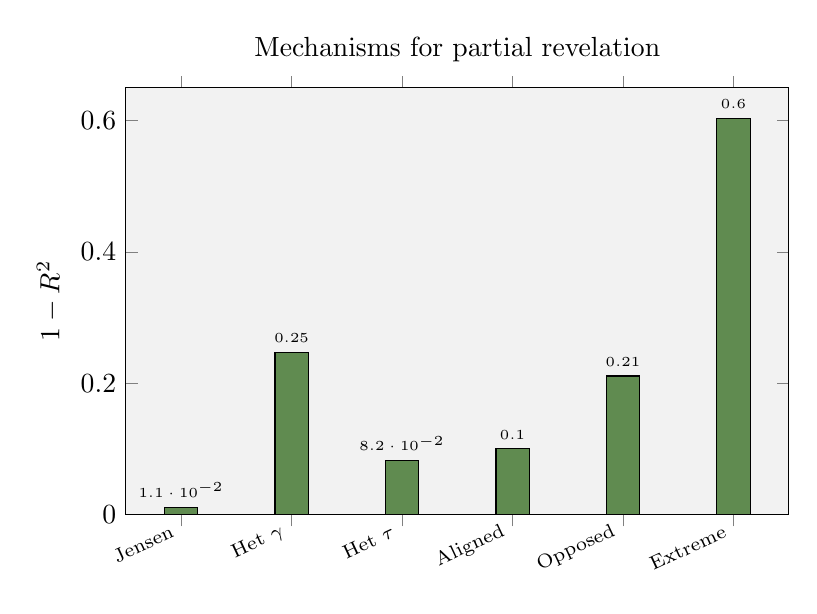
\begin{tikzpicture}
\begin{axis}[
  ybar, bar width=12pt,
  ymin=0, ymax=0.65,
  ylabel={$1-R^2$},
  width=10cm, height=7cm,
  axis background/.style={fill=black!5},
  symbolic x coords={Jensen,Het $\gamma$,Het $\tau$,Aligned,Opposed,Extreme},
  xtick=data, xticklabel style={font=\scriptsize,rotate=25,anchor=east},
  nodes near coords, every node near coord/.append style={font=\tiny},
  title={Mechanisms for partial revelation}]
\addplot[fill=green!70] coordinates {
  (Jensen,0.011) (Het $\gamma$,0.247) (Het $\tau$,0.082)
  (Aligned,0.100) (Opposed,0.211) (Extreme,0.604)};
\end{axis}
\end{tikzpicture}
\end{document}
